\newpage
\section{Aufbau und Durchführung}

\subsection{Aufbau}

\begin{figure}
    \begin{subfigure}{0.5\textwidth}
        \centering
        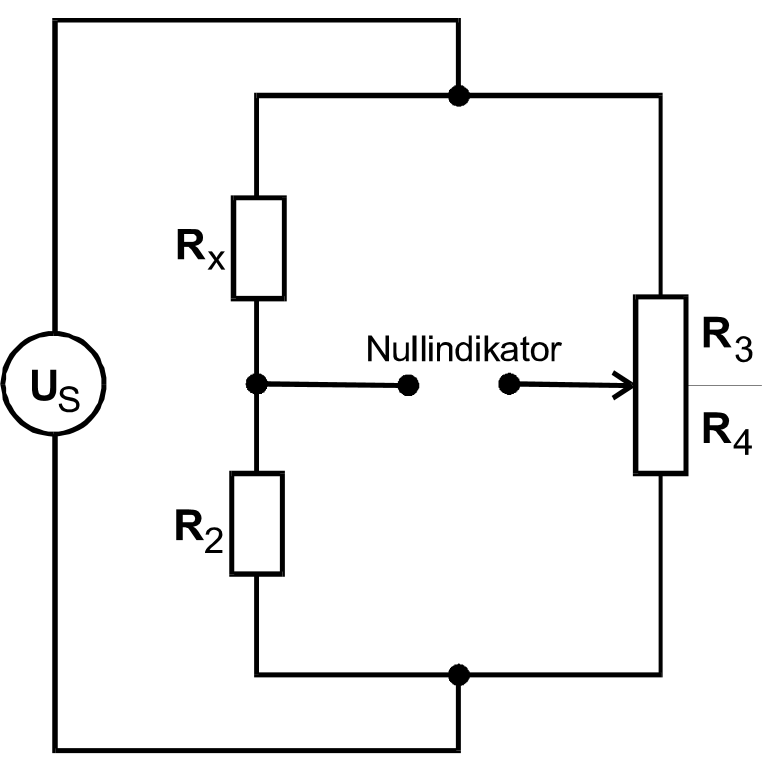
\includegraphics[height=4cm]{Bilder/Wheatstone.png}
        \caption{Wheatstonesche Brückenschaltung}
        \label{fig:Wheatstone}
    \end{subfigure}
    \begin{subfigure}{0.5\textwidth}
        \centering
        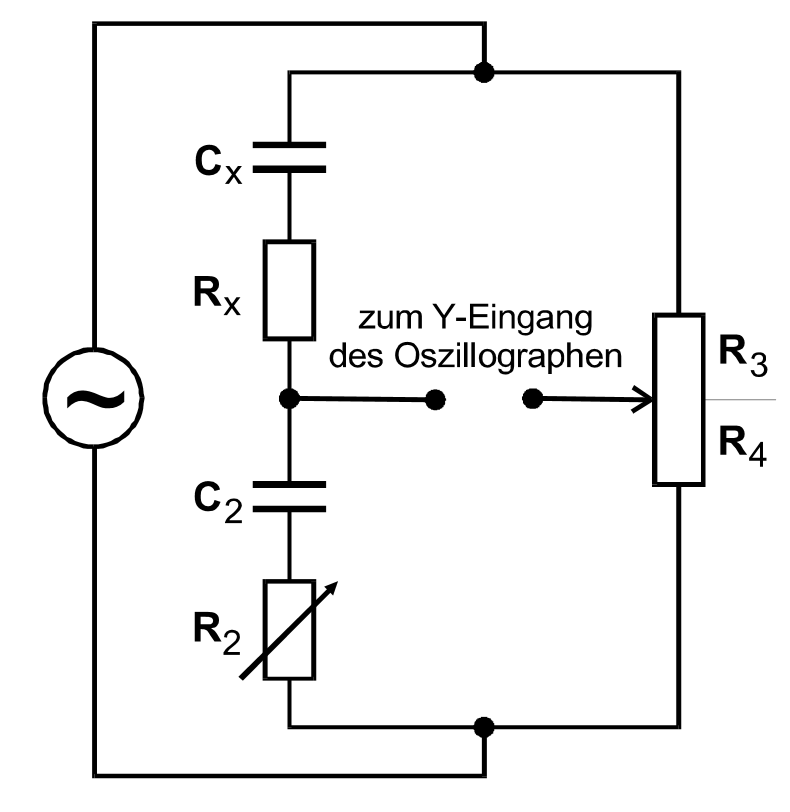
\includegraphics[height=4cm]{Bilder/Kapazitiv.png}
        \caption{Kapazitive Brückenschaltung}
        \label{fig:Kapazitiv}
    \end{subfigure}
    \begin{subfigure}{0.5\textwidth}
        \centering
        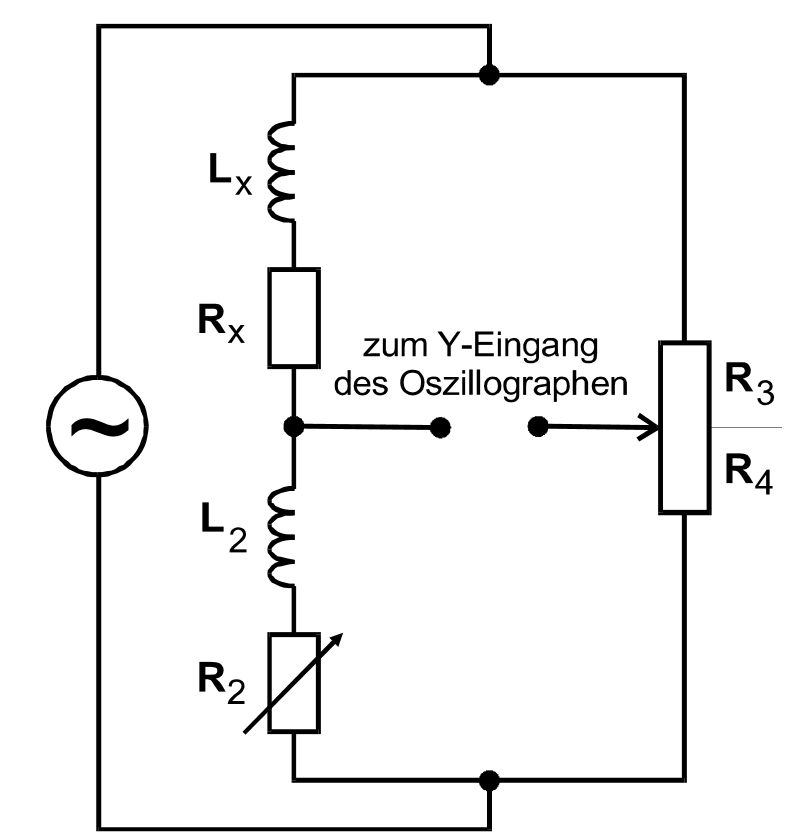
\includegraphics[height=4cm]{Bilder/Induktiv}
        \caption{Induktive Brückenschaltung}
        \label{fig:Induktiv}
    \end{subfigure}
    \begin{subfigure}{0.5\textwidth}
        \centering
        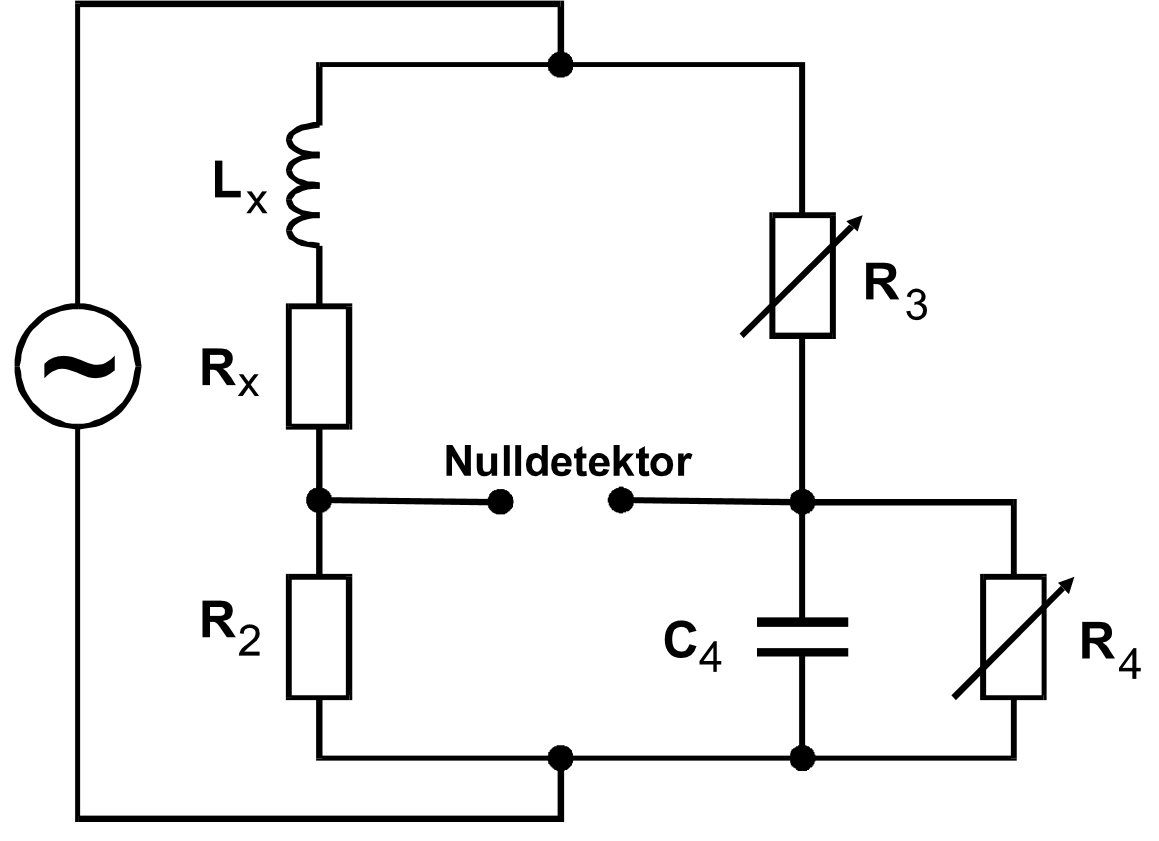
\includegraphics[height=4cm]{Bilder/Maxwell}
        \caption{Maxwellsche Brückenschaltung}
        \label{fig:Maxwell}
    \end{subfigure}
    \begin{subfigure}{0.5\textwidth}
        \centering
        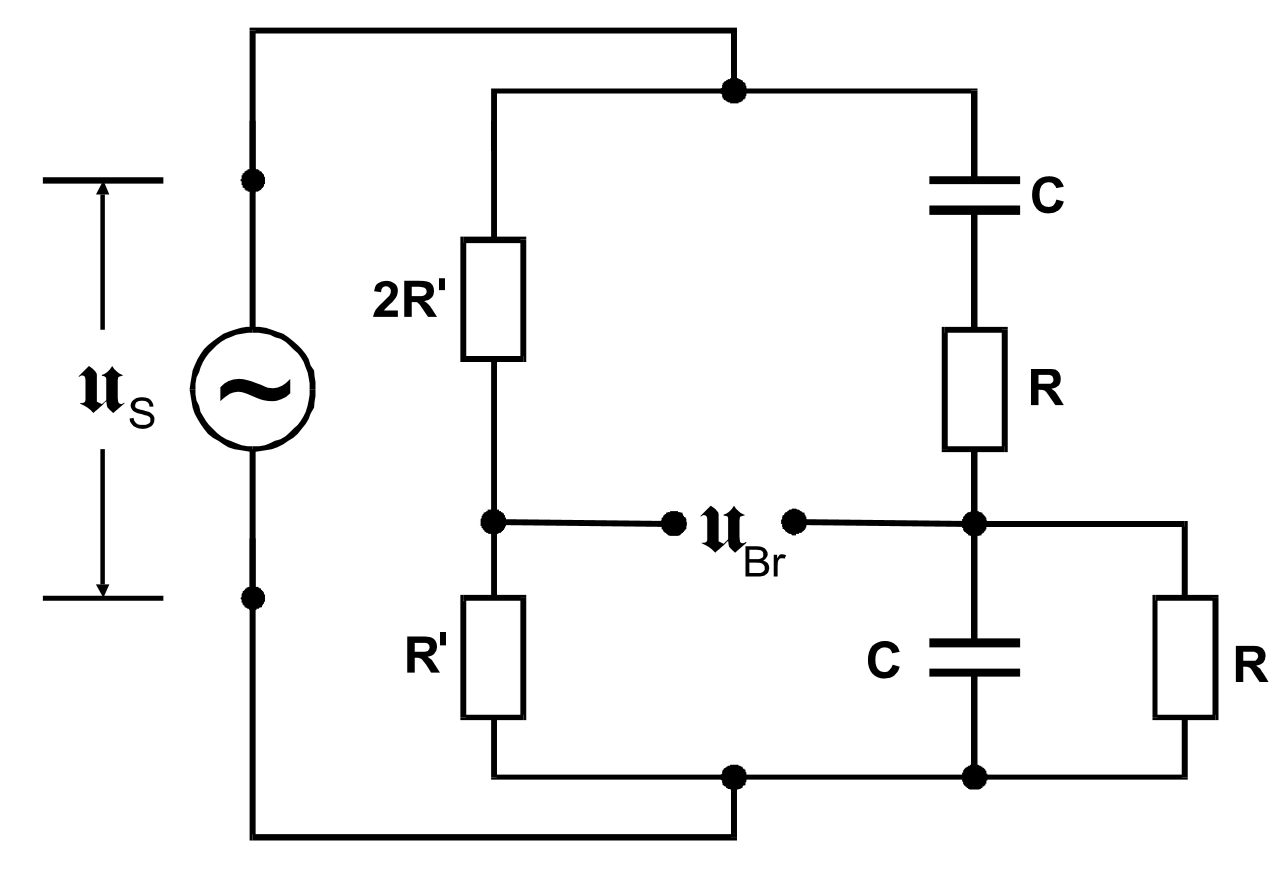
\includegraphics[height=4cm]{Bilder/Wien-Robinson}
        \caption{Wien-Robinson Brückenschaltung}
        \label{fig:Wien}
    \end{subfigure}
\end{figure}
\cite{v302}


\noindent Die Schaltkreise, entsrechend der Schaltbilder, werden
mit vorgefertigten Bauteilen zusammengefügt, wobei bestimmte Elemente unbekannte Werte haben.
Als Spannungsmessgerät wird ein Oszilloskop verwendet. $R_3$ und $R_4$ sind Potentiometer, wobei für
für die ersten drei Schaltungen gilt, dass $R_3+R_4=\qty{1000}{\ohm}$ ist.

\subsection{Durchführung}

\subsection{Wheatstonesche Brückenschaltung}
In der Wheatstoneschen Brückenschaltung (\ref{fig:Wheatstone}) müssen $R_3$ und $R_4$ variiert werden, 
bis im Oszilloskop die Brückenspannung auf $\qty{0}{\volt}$ fällt. Dann werden die entsprechenden Widerstände
notiert.

\subsection{Kapazitive Brückenschaltung}
In der Kapazitiven Schaltung wird die Brückenspannung nur auf ein Minimum gebracht, da störende Frequenzen in der 
Wechselspannung verhindern, dass diese auf $\qty{0}{\volt}$ fällt. Hierzu werden wieder $R_3$ und $R_4$ variiert.
Wenn das Minimum erreicht wurde, werden wieder die Widerstände notiert.

\subsection{Induktive Brückenschaltung}
Für die Induktive Brückenschaltung wird wie bei der kapazitiven die Brückenspannung wieder minimiert durch variieren
der bekannten Widerstände. Auch hier werden die Widersände notiert.

\subsection{Maxwellsche Brückenschaltung}
In der maxwellschen Brückenschaltung wird wieder die Brückenspannung minimiert mit $R_3$ und $R_4$, allerdings gilt hier
nichtmehr, dass deren Summe $\qty{1000}{\ohm}$ ergibt. Dabei ist es auch wichtig, dass man diese abwechselnd variiert, bis
das Ändern beider Widerstände die Spannung nicht mehr verringert. Die Widerstände werden notiert.

\subsection{Wien-Robinson Brückenschaltung}
Mit der Wien-Robinson Schaltung werden nun nur Bauteile mit bekannten Größen gewählt und die Frequenz $f$ 
der Eingangsspannung geändert. Zu jeder betrachteten Frequenz wird dann die Brückenspannung aufgetragen. Bis 
$\qty{500}{\hertz}$ wird die Frequenz in $\qty{50}{\hertz}$ Schritten aufgenommen und danach in $\qty{500}{\hertz}$
Schritten bis $\qty{5000}{\hertz}$.



\label{sec:Durchführung}
